\section{Geometric Series} \label{S:8.2.Geometric}

\vspace*{-14 pt}
\framebox{\hspace*{3 pt}
\parbox{\boxwidth}{\begin{goals}
\item What is a geometric series?
\item What is a partial sum of a geometric series? What is a simplified form of the $n$th partial sum of a geometric series?
\item Under what conditions does a geometric series converge? What is the sum of a convergent geometric series?
\end{goals}} \hspace*{3 pt}}

\subsection*{Introduction}

Many important sequences are generated through the process of addition.  In Preview Activity~\ref{PA:8.2}, we see a particular example of a special type of sequence that is connected to a sum.

\begin{pa} \label{PA:8.2}
Warfarin is an anticoagulant that prevents blood clotting; often it is prescribed to stroke victims in order  to help ensure blood flow. The level of warfarin has to reach a certain concentration in the blood in order to be effective. 

Suppose warfarin is taken by a particular patient in a 5 mg dose each day. The drug is absorbed by the body and some is excreted from the system between doses. Assume that at the end of a 24 hour period, 8\% of the drug remains in the body. Let $Q(n)$ be the amount (in mg) of warfarin in the body before the $(n+1)$st dose of the drug is administered.

\ba
\item Explain why $Q(1) = 5 \times 0.08$ mg.

\item Explain why $Q(2) = (5+Q(1)) \times 0.08$ mg. Then show that 
\[Q(2) = (5 \times 0.08)\left(1+0.08\right) \text{ mg}.\]

\item Explain why $Q(3) = (5+Q(2)) \times 0.08$ mg. Then show that
\[Q(3) = (5 \times 0.08)\left(1+0.08+0.08^2\right) \text{ mg}.\]

\item Explain why $Q(4) = (5+Q(3)) \times 0.08$ mg. Then show that
\[Q(4) = (5 \times 0.08)\left(1+0.08+0.08^2+0.08^3\right) \text{ mg}.\]

\item There is a pattern that you should see emerging. Use this pattern to find a formula for $Q(n)$, where $n$ is an arbitrary positive integer.

\item Complete Table \ref{T:8.2_Warfarin} with values of $Q(n)$ for the provided $n$-values (reporting $Q(n)$ to 10 decimal places). What appears to be happening to the sequence $Q(n)$ as $n $ increases?
\begin{table}[ht]
\begin{center}
\renewcommand{\arraystretch}{1.5}
\begin{tabular}{c|c}
$Q(1)$   & $0.40$ \\
$Q(2)$   & \\
$Q(3)$   &  \\
$Q(4)$   &  \\
$Q(5)$   &  \\
$Q(6)$   &  \\
$Q(7)$   &  \\
$Q(8)$   &  \\
$Q(9)$   &  \\
$Q(10)$  &  \\
\end{tabular}
\caption{Values of $Q(n)$ for selected values of $n$}
\label{T:8.2_Warfarin}
\end{center}
\end{table}


%\begin{itemize}
%\item After the first dose is administered, the body will absorb the drug and retain 8\% of the dose. So
%\[Q(1) = 5 \times 0.08 \text{ mg}.\]
%\item After the second dose is administered, the body will absorb the drug and retain 8\% of the dose, plus what remained in the body after the second dose. So
%\[Q(2) = 5 \times 0.08 + \left(0.08 \times 5\right) \times 0.08 = (5 \times 0.08)\left(1+0.08\right) \text{ mg}.\]
%\item After the third dose is administered, the body will absorb the drug and retain 8\% of the dose, plus what remained in the body after the third dose. So
%\[Q(3) = 5 \times 0.08 + \left(0.08 \times 5\right) \left(1+0.08\right)\times 0.08 = (5 \times 0.08)\left(1+0.08+0.08^2\right) \text{ mg}.\]
%\item After the fourth dose is administered, the body will absorb the drug and retain 8\% of the dose, plus what remained in the body after the fourth dose. So
%\[Q(4) = 5 \times 0.08 + \left(0.08 \times 5\right) \left(1+0.08+0.08^2\right)\times 0.08 = (5 \times 0.08)\left(1+0.08+0.08^2+0.08^3\right) \text{ mg}.\]
%\end{itemize}


%A pattern seems to be emerging. It appears that after the $n$th dose is administered, the body will absorb the drug and retain 8\% of the dose, plus what remained in the body after the $n$th dose and so
%\begin{equation} \label{eq:8.2_part_sum}
%Q(n)=(5 \times 0.08)\left(1+0.08+0.08^2+0.08^3+ \cdots + 0.08^{n-1}\right) \text{ mg}.
%\end{equation}

%*** begin comment ***

%Table \ref{T:8.2_Warfarin} gives the values of $Q(n)$ for a few selected values (to 10 decimal places) of $n$:
%\begin{table}[ht]
%\begin{center}
%\renewcommand{\arraystretch}{1.5}
%\begin{tabular}{c|c}
%$Q(1)$   & $0.40$ \\
%$Q(2)$   & $0.432$ \\
%$Q(3)$   & $0.43456$ \\
%$Q(4)$   & $0.4347648$ \\
%$Q(5)$   & $0.434781184$ \\
%$Q(6)$   & $0.4347824948$ \\
%$Q(7)$   & $0.4347825996$ \\
%$Q(8)$   & $0.4347826080$ \\
%$Q(9)$   & $0.4347826088$ \\
%$Q(10)$  & $0.4347826088$ \\
%\end{tabular}
%\caption{Values of $Q(n)$ for selected values of $n$}
%\label{T:8.2_Warfarin_Sol}
%\end{center}
%\end{table}
%We can plot the data points $(n,Q(n))$ and visualize the long-term behavior as shown in Figure \ref{F:8.2.Warfarin}

%\begin{figure}[h]
%\begin{center}
%\resizebox{!}{1.5in}{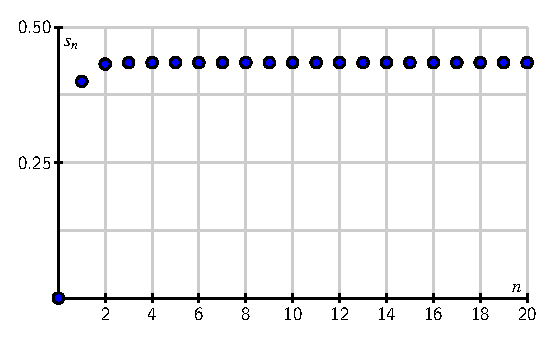
\includegraphics{figures/8_2_Warfarin.eps}}
%\caption{The points $(n, Q(n))$ for $n$ from 1 to 20}
%\label{F:8.2.Warfarin}
%\end{center}
%\end{figure}

%The data and the graph appears to indicate there is a long-term level of Warfarin that remains in the blood, or a limit to the sequence of values $Q(n)$ as $n$ goes to infinity. The data approximates this ling-term level, but with a little more work we can find the exact level of Warfarin in the blood.

%*** end comment ****

\ea

\end{pa}
\afterpa 

\subsection*{Geometric Sums}

In Preview Activity \ref{PA:8.2} we encountered the sum
\[(5 \times 0.08)\left(1+0.08+0.08^2+0.08^3+ \cdots + 0.08^{n-1}\right).\]
In order to evaluate the long-term level of Warfarin in the patient's system, we will want to fully understand the sum in this expression. This sum has the form
\begin{equation} \label{eq:8.2_part_sum_geometric_1}
a+ar+ar^2+ \cdots + ar^{n-1}
\end{equation}
where $a=5 \times 0.08$ and $r=0.08$. Such a sum is called a \emph{geometric sum}\index{geometric sum} with ratio $r$. We will analyze this sum in more detail in the next activity.

\begin{activity} \label{8.2.Act1} Let $a$ and $r$ be real numbers (with $r \ne 1$) and let
\[S_n = a+ar+ar^2 + \cdots + ar^{n-1}.\]
In this activity we will find a shortcut formula for $S_n$ that does not involve a sum of $n$ terms.
\ba
\item Multiply $S_n$ by $r$. What does the resulting sum look like?


\item Subtract $rS_n$ from $S_n$ and explain why
\begin{equation} \label{eq:8.2.1_partial_geometric_sum}
S_n - rS_n = a - ar^n.
\end{equation}


\item Solve equation (\ref{eq:8.2.1_partial_geometric_sum}) for $S_n$ to find a simple formula for $S_n$ that does not involve adding $n$ terms.


\ea
\end{activity}

\begin{smallhint}
\ba
	\item Small hints for each of the prompts above.
\ea
\end{smallhint}
\begin{bighint}
\ba
	\item Big hints for each of the prompts above.
\ea
\end{bighint}
\begin{activitySolution}
\ba
	\item Note that
\[rS_n = ar+ar^2+ar^3 + \cdots + ar^n.\]
    \item When we subtract $rS_n$ from $S_n$ the middle terms all cancel and we are left with
\begin{align*}
S_n - rS_n &= \left(a+ar+ar^2 + \cdots + ar^{n-1}\right) - \left(ar+ar^2+ar^3 + \cdots + ar^n\right) \\
    &=a + (ar-ar) + \left(ar^2-ar^2\right) + \cdots + \left(ar^{n-1}-ar^{n-1}\right) - ar^n \\
    &= a - ar^n.
    \end{align*}
    \item Factoring $S_n$ from left hand side and dividing gives us a formula for $S_n$:
\begin{align*}
S_n(1-r) &= a - ar^n \\
S_n &= a\frac{1-r^n}{1-r}.
\end{align*}

\ea
\end{activitySolution}
\aftera 

We can summarize the result of Activity \ref{8.2.Act1} in the following way.

\vspace*{5pt}
\nin \framebox{\hspace*{3 pt}
\parbox{\boxwidth}{
A geometric sum $S_n$ is a sum of the form
\begin{equation} \label{eq:8.2_geometric_sum}
S_n = a + ar + ar^2 + \cdots + ar^{n-1},
\end{equation}
where $a$ and $r$ are real numbers such that $r \ne 1$. The geometric sum $S_n$ can be written more simply as
\begin{equation} \label{eq:8.2_part_sum_geometric}
S_n = a+ar+ar^2+ \cdots + ar^{n-1} = \frac{a(1-r^n)}{1-r}.
\end{equation}
} \hspace*{3 pt}}
\vspace*{1pt}

We now apply equation (\ref{eq:8.2_part_sum_geometric}) to the example involving warfarin from Preview Activity~\ref{PA:8.2}. Recall that
\[Q(n)=(5 \times 0.08)\left(1+0.08+0.08^2+0.08^3+ \cdots + 0.08^{n-1}\right) \text{ mg},\]
so $Q(n)$ is a geometric sum with $a=5 \times 0.08 = 0.4$ and $r = 0.08$. Thus,
\[Q(n) = 0.4\left(\frac{1-0.08^n}{1-0.08}\right) = \frac{1}{2.3} \left(1-0.08^n\right).\]
Notice that as $n$ goes to infinity, the value of $0.08^n$ goes to 0. So,
\[\lim_{n \to \infty} Q(n) = \lim_{n \to \infty}  \frac{1}{2.3} \left(1-0.08^n\right) = \frac{1}{2.3} \approx 0.435.\]
Therefore, the long-term level of Warfarin in the blood under these conditions is $\frac{1}{2.3}$, which is approximately 0.435 mg.

To determine the long-term effect of Warfarin, we considered a geometric sum of $n$ terms, and then considered what happened as $n$ was allowed to grow without bound.  In this sense, we were actually interested in an infinite geometric sum (the result of letting $n$ go to infinity in the finite sum).  We call such an infinite geometric sum a \emph{geometric series}. \index{geometric series} \index{series!geometric}

\begin{definition}  A geometric series is an infinite sum of the form
\begin{equation} \label{eq:8.2_geometric_series}
a + ar + ar^2 + \cdots = \sum_{n=0}^{\infty} ar^n.
\end{equation}
\end{definition}
The value of $r$ in the geometric series (\ref{eq:8.2_geometric_series}) is called the \emph{common ratio} \index{geometric series!common ratio} of the series because the ratio of the ($n+1$)st term $ar^n$ to the $n$th term $ar^{n-1}$ is always $r$.

Geometric series are very common in mathematics and arise naturally in many different situations. As a familiar example, suppose we want to write the number with repeating decimal expansion
\[N=0.1212\overline{12}\]
as a rational number.
Observe that
\begin{align*}
N &=  0.12 + 0.0012 + 0.000012 + \cdots \\
    &= \left(\frac{12}{100}\right) + \left(\frac{12}{100}\right)\left(\frac{1}{100}\right) + \left(\frac{12}{100}\right)\left(\frac{1}{100}\right)^2 + \cdots,
\end{align*}
which is an infinite geometric series with $a=\frac{12}{100}$ and $r = \frac{1}{100}$.   In the same way that we were able to find a shortcut formula for the value of a (finite) geometric sum, we would like to develop a formula for the value of a (infinite) geometric series.  We explore this idea in the following activity.

\begin{activity} \label{8.2.Act2} Let $r \ne 1$ and $a$ be real numbers and let
\[S = a+ar+ar^2 + \cdots ar^{n-1} + \cdots \]
be an infinite geometric series. For each positive integer $n$, let
\[S_n = a+ar+ar^2 + \cdots + ar^{n-1}.\]
Recall that
\[S_n = a\frac{1-r^n}{1-r}.\]
\ba
\item What should we allow $n$ to approach in order to have $S_n$ approach $S$?

\item What is the value of  $\ds \lim_{n \to \infty} r^n$ for
\begin{itemize}
\item $|r| > 1$?
\item $|r| < 1$?
\end{itemize}
Explain.



\item If $|r| < 1$, use the formula for $S_n$ and your observations in (a) and (b) to explain why $S$ is finite and find a resulting formula for $S$.



\ea
\end{activity}

\begin{smallhint}
\ba
	\item Small hints for each of the prompts above.
\ea
\end{smallhint}
\begin{bighint}
\ba
	\item Big hints for each of the prompts above.
\ea
\end{bighint}
\begin{activitySolution}
\ba
	\item It is the case that
\[S = \lim_{n \to \infty} S_n.\]
    \item 
\begin{itemize}
\item If $r > 1$, then $\ds \lim_{n \to \infty} r^n = \infty$.
\item If $0 < r < 1$, then $\ds \lim_{n \to \infty} r^n = 0$.
\end{itemize}
    \item Since
\[S = \lim_{n \to \infty} S_n = \lim_{n \to \infty} a\frac{1-r^n}{1-r}\]
and
\[\lim_{n \to \infty} r^n = 0\]
for $0 < r < 1$, we conclude that
\[S = \lim_{n \to \infty} a\frac{1-r^n}{1-r} = \frac{a}{1-r}\]
when $0 < r < 1$.


\ea
\end{activitySolution}
\aftera 

From our work in Activity \ref{8.2.Act2}, we can now find the value of the geometric series $N = \left(\frac{12}{100}\right) + \left(\frac{12}{100}\right)\left(\frac{1}{100}\right) + \left(\frac{12}{100}\right)\left(\frac{1}{100}\right)^2 + \cdots.$  In particular, using $a = \frac{12}{100}$ and $r = \frac{1}{100}$, we see that
\[N = \frac{12}{100} \left(\frac{1}{1-\frac{1}{100}}\right) = \frac{12}{100} \left(\frac{100}{99}\right) = \frac{4}{33}.\]

It is important to notice that a geometric sum is simply the sum of a finite number of terms of a geometric series. In other words, the geometric sum $S_n$ for the geometric series
\[\sum_{k=0}^{\infty} ar^k\]
is
\[S_n = a+ar+ar^2 + \cdots + ar^{n-1} = \sum_{k=0}^{n-1} ar^k.\]
We also call this sum $S_n$ the $n$th \emph{partial sum}\index{partial sum} of the geometric series. We summarize our recent work with geometric series as follows.

\vspace*{5pt}
\nin \framebox{\hspace*{3 pt}
\parbox{\boxwidth}{
\begin{itemize}
\item A geometric series is an infinite sum of the form
\begin{equation} \label{eq:8.2_geometric_series_2}
a + ar + ar^2 + \cdots = \sum_{n=0}^{\infty} ar^n,
\end{equation}
where $a$ and $r$ are real numbers such that $r \ne 0$.
\item The $n$th partial sum $S_n$ of the geometric series is
\[S_n = a+ar+ar^2+ \cdots + ar^{n-1}.\]
\item If $|r| < 1$, then using the fact that $S_n = a\frac{1-r^n}{1-r}$, it follows that the sum $S$ of the geometric series (\ref{eq:8.2_geometric_series_2}) is
\[S = \lim_{n \to \infty} S_n = \lim_{n \to \infty} a\frac{1-r^n}{1-r} = \frac{a}{1-r}\]
\end{itemize}
} \hspace*{3 pt}}
\vspace*{1pt}

\begin{activity} \label{8.2.Act3} The formulas we have derived for the geometric series and its partial sum so far have assumed we begin indexing our sums at $n=0$. If instead we have a sum that does not begin at $n=0$, we can factor out common terms and use our established formulas.  This process is illustrated in the examples in this activity.
\ba
\item Consider the sum
\[ \sum_{k=1}^{\infty} (2)\left(\frac{1}{3}\right)^k = (2)\left(\frac{1}{3}\right) + (2)\left(\frac{1}{3}\right)^2 + (2)\left(\frac{1}{3}\right)^3 + \cdots .\]
Remove the common factor of $(2)\left(\frac{1}{3}\right)$ from each term and hence find the sum of the series. 

\item Next let $a$ and $r$ be real numbers with $-1<r<1$. Consider the sum  
\[\sum_{k=3}^{\infty} ar^k = ar^3+ar^4+ar^5 + \cdots.\]
Remove the common factor of $ar^3$ from each term and find the sum of the series. 

\item Finally, we consider the most general case. Let $a$ and $r$ be real numbers with $-1<r<1$, let $n$ be a positive integer, and consider the sum
\[ \sum_{k=n}^{\infty} ar^k = ar^n+ar^{n+1}+ar^{n+2} + \cdots .\]
Remove the common factor of $ar^n$ from each term to find the sum of the series. 

\ea
\end{activity}

\begin{smallhint}
\ba
	\item Small hints for each of the prompts above.
\ea
\end{smallhint}
\begin{bighint}
\ba
	\item Big hints for each of the prompts above.
\ea
\end{bighint}
\begin{activitySolution}
\ba
	\item Factoring out $(2)\left(\frac{1}{3}\right)$ gives us
\begin{align*}
(2)\left(\frac{1}{3}\right) \left[1 + \left(\frac{1}{3}\right) + \left(\frac{1}{3}\right)^2 + \cdots \right] &= (2)\left(\frac{1}{3}\right)\sum_{k=0}^{\infty} \left(\frac{1}{3}\right)^k \\
    &= (2)\left(\frac{1}{3}\right) \left(\frac{1}{1-\frac{1}{3}}\right) \\
    &= (2)\left(\frac{1}{3}\right) \left(\frac{3}{2}\right)\\
    &=  4.
\end{align*}
    \item Factoring out $ar^3$ gives us
\begin{align*}
ar^3+ar^4+ar^5 + \cdots &= ar^3\left(1+r+r^2+ \cdots \right) \\
    &= ar^3\sum_{k=0}^{\infty} r^k \\
    &= ar^3 \left(\frac{1}{1-r}\right) \\
    &= \frac{ar^3}{1-r}.
\end{align*}
    \item Factoring out $ar^n$ gives us
\begin{align*}
ar^n+ar^{n+1}+ar^{n+2} + \cdots &= ar^n\left(1+r+r^2+ \cdots \right) \\
    &= ar^n\sum_{k=0}^{\infty} r^k \\
    &= ar^n \left(\frac{1}{1-r}\right) \\
    &= \frac{ar^n}{1-r}.
\end{align*}
\ea
\end{activitySolution}
\aftera 

%\nin \framebox{\hspace*{3 pt}
%\parbox{6.25 in}{
\begin{summary}
\item A geometric series is an infinite sum of the form
\[\sum_{k=0}^{\infty} ar^k\]
where $a$ and $r$ are real numbers and $r \neq 0$.
\item For the geometric series $\ds \sum_{k=0}^{\infty} ar^k$, its $n$th partial sum is
\[S_n = \sum_{k=0}^{n-1} ar^k.\]
An alternate formula for the $n$th partial sum is
\[S_n = a \frac{1-r^n}{1-r}.\]
Whenever $|r| < 1$, the infinite geometric series $\sum_{k=0}^{\infty} ar^k$ has the finite sum $\frac{a}{1-r}$.
\end{summary}
%} \hspace*{3 pt}}

\nin \hrulefill

\begin{exercises}
\item There is an old question that is often used to introduce the power of geometric growth. Here is one version. Suppose you are hired for a one month (30 days, working every day) job and are given two options to be paid.
\begin{description}
\item[Option 1.] You can be paid \$500 per day or
\item[Option 2.] You can be paid 1 cent the first day, 2 cents the second day, 4 cents the third day, 8 cents the fourth day, and so on, doubling the amount you are paid each day.
\end{description}

    \ba
	\item How much will you be paid for the job in total under Option 1?

    \item Complete Table \ref{PA8.2:geometric} to determine the pay you will receive under Option 2 for the first 10 days.
    \begin{table}[h]
    \begin{center}
    \renewcommand{\arraystretch}{1.5}
    \begin{tabular}{ccc} \hline
    Day     &Pay on this day    &Total amount paid to date \\ \hline
    $1$     &$\$0.01$           &$\$0.01$       \\ \hline
    $2$     &$\$0.02$           &$\$0.03$       \\ \hline
    $3$     &                   &       \\ \hline
    $4$     &                   &       \\ \hline
    $5$     &                   &       \\ \hline
    $6$     &                   &       \\ \hline
    $7$     &                   &       \\ \hline
    $8$     &                   &       \\ \hline
    $9$     &                   &       \\ \hline
    $10$    &                   &       \\ \hline
    \end{tabular}
    \caption{Option 2 payments}
    \label{PA8.2:geometric}
    \end{center}
    \end{table}


    \item Find a formula for the amount paid on day $n$, as well as for the total amount paid by day $n$. Use this formula to determine which option (1 or 2) you should take.

\begin{exerciseSolution}

On day $n$ you are paid $0.01\left(2^{n-1}\right)$ dollars and the total amount paid is $\$0.01\left(2^n-1\right)$. So on day 30 under Option 2 the total payment will be
\[\$0.01\left(2^{30}-1\right) = \$10,737,418.23,\]
so Option 2 is definitely the better deal.

\end{exerciseSolution}



\ea

\item  Suppose you drop a golf ball onto a hard surface from a height $h$. The collision with the ground causes the ball to lose energy and so it will not bounce back to its original height. The ball will then fall again to the ground, bounce back up, and continue. Assume that at each bounce the ball rises back to a height $\frac{3}{4}$ of the height from which it dropped. Let $h_n$ be the height of the ball on the $n$th bounce, with $h_0 = h$. In this exercise we will determine the distance traveled by the ball and the time it takes to travel that distance.

\ba
\item Determine a formula for $h_1$ in terms of $h$.

\begin{exerciseSolution}

Since the ball bounces back 3/4 of the original height, we have
\[h_1 = \left(\frac{3}{4}\right)h.\]

\end{exerciseSolution}

\item Determine a formula for $h_2$ in terms of $h$.

\begin{exerciseSolution}

Since the ball bounces back 3/4 of the original height, we have
\[h_2 = \left(\frac{3}{4}\right)h_1 = \left(\frac{3}{4}\right)^2h.\]

\end{exerciseSolution}

\item Determine a formula for $h_3$ in terms of $h$.

\begin{exerciseSolution}

Since the ball bounces back 3/4 of the original height, we have
\[h_3 = \left(\frac{3}{4}\right)h_2 = \left(\frac{3}{4}\right)^3h.\]

\end{exerciseSolution}

\item Determine a formula for $h_n$ in terms of $h$.

\begin{exerciseSolution}

Since the ball bounces back 3/4 of the original height, we have
\[h_n = \left(\frac{3}{4}\right)h_{n-1} = \left(\frac{3}{4}\right)^nh.\]

\end{exerciseSolution}

\item Write an infinite series that represents the total distance traveled by the ball. Then determine the sum of this series.

\begin{exerciseSolution}

The distance traveled by the ball is
\begin{align*}
h+2[h_1+h_2+ \cdots ] &= h + 2 \left[ \left(\frac{3}{4}\right)^2h + \left(\frac{3}{4}\right)^2h + \left(\frac{3}{4}\right)^2h + \cdots \right] \\
    &= h + 2\left(\frac{3}{4}\right)h \left[1 + \left(\frac{3}{4}\right) + \left(\frac{3}{4}\right)^2 + \cdots \right]
    &= h + \left(\frac{3}{2}\right)h \sum_{n = 0}^{\infty} \left(\frac{3}{4}\right)^n \\
    &= h + \left(\frac{3}{2}\right)h \left(\frac{1}{1-3/4}\right) \\
    &= h + \left(\frac{3}{2}\right)h (4) \\
    &= h + 6h \\
    &= 7h.
\end{align*}
So no matter what the initial height of the ball, the ball will bounce infinitely many times but only travel a finite distance.

\end{exerciseSolution}

\item Next, let's determine the total amount of time the ball is in the air.
    \begin{itemize}
    \item[(i)] When the ball is dropped from a height $H$, if we assume the only force acting on it is the acceleration due to gravity, then the height of the ball at time $t$ is given by
\[H - \frac{1}{2}gt^2.\]
Use this formula to determine the time it takes for the ball to hit the ground after being dropped from height $H$.

    \item[(ii)] Use your work in the preceding item, along with that in (a)-(e) above to determine the total amount of time the ball is in the air.

    \end{itemize}

\ea


\item Suppose you play a game with a friend that involves rolling a standard six-sided die. Before a player can participate in the game, he or she must roll a six with the die. Assume that you roll first and that you and your friend take alternate rolls. In this exercise we will determine the probability that you roll the first six. 
    \ba
    \item Explain why the probability of rolling a six on any single roll (including your first turn) is $\frac{1}{6}$. 
    
    \item If you don't roll a six on your first turn, then in order for you to roll the first six on your second turn, both you and your friend had to fail to roll a six on your first turns, and then you had to succeed in rolling a six on your second turn. Explain why the probability of this event is 
        \[\left(\frac{5}{6}\right)\left(\frac{5}{6}\right)\left(\frac{1}{6}\right) = \left(\frac{5}{6}\right)^2\left(\frac{1}{6}\right).\]
                
    \item Now suppose you fail to roll the first six on your second turn. Explain why the probability is 
        \[\left(\frac{5}{6}\right)\left(\frac{5}{6}\right)\left(\frac{5}{6}\right)\left(\frac{5}{6}\right)\left(\frac{1}{6}\right) = \left(\frac{5}{6}\right)^4\left(\frac{1}{6}\right)\]
        that you to roll the first six on your third turn. 
        
    \item The probability of you rolling the first six is the probability that you roll the first six on your first turn plus the probability that you roll the first six on your second turn plus the probability that your roll the first six on your third turn, and so on. Explain why this probability is 
        \[\frac{1}{6} + \left(\frac{5}{6}\right)^2\left(\frac{1}{6}\right) +  \left(\frac{5}{6}\right)^4\left(\frac{1}{6}\right) + \cdots.\]
        Find the sum of this series and determine the probability that you roll the first six. 
        
    \ea

  \item The goal of a federal government stimulus package is to positively affect the economy. Economists and politicians quote numbers like ``$k$ million jobs and a net stimulus to the economy of $n$ billion of dollars.'' Where do they get these numbers? Let's consider one aspect of a stimulus package: tax cuts. Economists understand that tax cuts or rebates can result in long-term spending that is many times the amount of the rebate. For example, assume that for a typical person, 75\% of her entire income is spent (that is, put back into the economy). Further, assume the government provides a tax cut or rebate that totals $P$ dollars for each person.
      \ba
      \item The tax cut of $P$ dollars is income for its recipient. How much of this tax cut will be spent?

\begin{exerciseSolution}

Given that 75\% of income is spent, this tax cut/rebate will result in $0.75P$ dollars spent.

\end{exerciseSolution}

    \item In this simple model, we will say that the spent portion of the tax cut/rebate from part (a) then becomes income for another person who, in turn, spends 75\% of this income. After this ``second round" of spent income, how many total dollars have been added to the economy as a result of the original tax cut/rebate?

\begin{exerciseSolution}

The amount of money introduced into the economy is the amount $0.75P$ after the original cut plus 75\% of that income from spending. So the total amount of money added to the economy is
\[0.75P + 0.75(0.75P) = 0.75P(1+0.75)\]
dollars.

\end{exerciseSolution}

    \item This second round of spending becomes income for another group who spend 75\% of this income, and so on. In economics this is called the \emph{multiplier effect}. Explain why an original tax cut/rebate of $P$ dollars will result in multiplied spending of
\[0.75P(1+0.75+0.75^2+ \cdots ).\]
dollars.

\begin{exerciseSolution}

The $n-1$st round of spending will result in income of $0.75^nP$ dollars, of which $75\%$ or $0.75^{n+1}P$ will be spent. So each round of spending adds a factor to the total amount, giving us a total amount of spending in the economy of
\[0.75P + 0.75^2P + 0.75^2P + \cdots = 0.75P(1+0.75+0.75^2+ \cdots )\]
dollars.

\end{exerciseSolution}

    \item Based on these assumptions, how much stimulus will a 200 billion dollar tax cut/rebate to consumers add to the economy, assuming consumer spending remains consistent forever.

\begin{exerciseSolution}

Using the sum of a geometric series with ratio $0.75$ shows that
\begin{align*}
0.75P(1+0.75+0.75^2+ \cdots ) &= 0.75P\left( \frac{1}{1-0.75} \right) \\
        &= 0.75P(4) \\
        &= 3P.
\end{align*}
So a stimulus of 200 billion dollars adds 600 billion dollars to the economy.

\end{exerciseSolution}

    \ea


\item Like stimulus packages, home mortgages and foreclosures also impact the economy. A problem for many borrowers is the adjustable rate mortgage, in which the interest rate can change (and usually increases) over the duration of the loan, causing the monthly payments to increase beyond the ability of the borrower to pay. Most financial analysts recommend fixed rate loans, ones for which the monthly payments remain constant throughout the term of the loan. In this exercise we will analyze fixed rate loans.

    When most people buy a large ticket item like car or a house, they have to take out a loan to make the purchase. The loan is paid back in monthly installments until the entire amount of the loan, plus interest, is paid. With a loan, we borrow money, say $P$ dollars (called the principal), and pay off the loan at an interest rate of $r$\%. To pay back the loan we make regular monthly payments, some of which goes to pay off the principal and some of which is charged as interest. In most cases, the interest is computed based on the amount of principal that remains at the beginning of the month. We assume a fixed rate loan, that is one in which we make a constant monthly payment $M$ on our loan, beginning in the original month of the loan.

    Suppose you want to buy a house. You have a certain amount of money saved to make a down payment, and you will borrow the rest to pay for the house. Of course, for the privilege of loaning you the money, the bank will charge you interest on this loan, so the amount you pay back to the bank is more than the amount you borrow. In fact, the amount you ultimately pay depends on three things: the amount you borrow (called the \emph{principal}), the interest rate, and the length of time you have to pay off the loan plus interest (called the \emph{duration} of the loan). For this example, we assume that the interest rate is fixed at $r$\%.

    To pay off the loan, each month you make a payment of the same amount (called \emph{installments}). Suppose we borrow $P$ dollars (our principal) and pay off the loan at an interest rate of $r$\% with regular monthly installment payments of $M$ dollars. So in month 1 of the loan, before we make any payments, our principal is $P$ dollars. Our goal in this exercise is to find a formula that relates these three parameters to the time duration of the loan.

    We are charged interest every month at an annual rate of $r$\%, so each month we pay $\frac{r}{12}$\% interest on the principal that remains. Given that the original principal is $P$ dollars, we will pay $\left(\frac{0.0r}{12}\right)P$ dollars in interest on our first payment. Since we paid $M$ dollars in total for our first payment, the remainder of the payment ($M-\left(\frac{r}{12}\right)P$) goes to pay down the principal. So the principal remaining after the first payment (let's call it $P_1$) is the original principal minus what we paid on the principal, or
    \[P_1 = P - \left( M - \left(\frac{r}{12}\right)P\right) = \left(1 + \frac{r}{12}\right)P - M.\]
    As long as $P_1$ is positive, we still have to keep making payments to pay off the loan.

    \ba
    \item Recall that the amount of interest we pay each time depends on the principal that remains. How much interest, in terms of $P_1$ and $r$, do we pay in the second installment?

\begin{exerciseSolution}
\vs

In the second installment, we are charged $\left(\frac{r}{12}\right)P_1$ dollars in interest.

\vs

\end{exerciseSolution}

    \item How much of our second monthly installment goes to pay off the principal? What is the principal $P_2$, or the balance of the loan, that we still have to pay off after making the second installment of the loan? Write your response in the form $P_2 = ( \ )P_1 - ( \ )M$, where you fill in the parentheses.

\begin{exerciseSolution}
\vs
The amount of our payment $M$ that doesn't go toward interest is applied toward the principal. So we reduce our principal by $M-\left(\frac{r}{12}\right)P_1$ dollars. Therefore, the balance of our loan after the second installment is
\[P_2 = P_1 - \left( M - \left(\frac{r}{12}\right)P_1 \right) = \left(1 + \frac{r}{12}\right)P_1 - M.\]

\vs
\end{exerciseSolution}
	
    \item Show that $P_2 = \left(1 + \frac{r}{12}\right)^2P - \left[1 + \left(1+\frac{r}{12}\right)\right] M$.

\begin{exerciseSolution}
\vs

We know $P_2 = \left(1 + \frac{r}{12}\right)P_1 - M$, so we substitute for $P_1$ and simplify:
\begin{align*}
P_2 &= \left(1 + \frac{r}{12}\right)P_1 - M \\
	&= \left(1 + \frac{r}{12}\right)\left[\left(1+\frac{r}{12}\right)P - M\right] - M \\
	&= \left(1 + \frac{r}{12}\right)^2P - \left[1 + \left(1+\frac{r}{12}\right)\right] M.
\end{align*}

\vs
\end{exerciseSolution}

    \item Let $P_3$ be the amount of principal that remains after the third installment. Show that
\[P_3 = \left(1 + \frac{r}{12}\right)^3P - \left[1 + \left(1+\frac{r}{12}\right) + \left(1+\frac{r}{12}\right)^2 \right] M.\]

\begin{exerciseSolution}
\vs

For the third payment we are charged $\left(\frac{r}{12}\right)P_2$ dollars in interest. So $M-\left(\frac{r}{12}\right)P_2$ dollars goes toward paying down the principal. Then
\[P_3 = P_2 - \left( M - \left(\frac{r}{12}\right)P_2 \right) = \left(1 + \frac{r}{12}\right)P_2 - M.\]

So $P_3 = \left(1 + \frac{r}{12}\right)P_2 - M$, so we substitute for $P_2$ and simplify:
\begin{align*}
P_3 &= \left(1 + \frac{r}{12}\right)P_2 - M \\
	&=  \left(1 + \frac{r}{12}\right)\left[\left(1 + \frac{r}{12}\right)^2P - \left[1 + \left(1+\frac{r}{12}\right)\right] M\right] - M\\
	&= \left(1 + \frac{r}{12}\right)^3P - \left[1 + \left(1+\frac{r}{12}\right) + \left(1+\frac{r}{12}\right)^2 \right] M.
\end{align*}

\vs
\end{exerciseSolution}

    \item If we continue in the manner described in the problems above, then the remaining principal of our loan after $n$ installments is
\begin{equation} \label{eq:loan_1}
P_n = \left(1 + \frac{r}{12}\right)^nP - \left[\displaystyle \sum_{k=0}^{n-1} \left(1+\frac{r}{12}\right)^k \right] M.
\end{equation}

This is a rather complicated formula and one that is difficult to use. However, we can simplify the sum if we recognize part of  it as a partial sum of a geometric series. Find a formula for the sum
\begin{equation} \label{eq:part_sum}
\displaystyle \sum_{k=0}^{n-1} \left(1+\frac{r}{12}\right)^k.
\end{equation}
and then a general formula for $P_n$ that does not involve a sum.

\begin{exerciseSolution}

The sum in (\ref{eq:part_sum}) is a partial sum of the geometric series with ratio $1+\frac{r}{12}$. So formula (\ref{eq:8.2_part_sum_geometric}) shows that the partial sum $\displaystyle \sum_{k=0}^{n-1} \left(1+\frac{r}{12}\right)^k$ is equal to

\begin{align*}
\displaystyle \sum_{k=0}^{n-1} \left(1+\frac{r}{12}\right)^k &= \frac{1-\left(1+\frac{r}{12}\right)^n}{1-\left(1+\frac{r}{12}\right)} \\
	&= \left(\frac{12}{r}\right) \left(\left(1+\frac{r}{12}\right)^n - 1\right).
\end{align*}

Now we can determine that the remaining principal after $n$ installments is
\begin{align*}
P_n &= \left(1 + \frac{r}{12}\right)^nP - \left[\left(\frac{12}{r}\right) \left(\left(1+\frac{r}{12}\right)^n - 1\right) \right] M \\
	&= P \left(1+\frac{r}{12}\right)^n - \left(\frac{12M}{r}\right) \left( \left(1+\frac{r}{12}\right)^n - 1\right).
\end{align*}

\end{exerciseSolution}

    \item It is usually more convenient to write our formula for $P_n$ in terms of years rather than months. Show that $P(t)$, the principal remaining after $t$ years, can be written as
\begin{equation} \label{eq:loan2}
P(t) = \left(P - \frac{12M}{r}\right)\left(1+\frac{r}{12}\right)^{12t} + \frac{12M}{r}.
\end{equation}

\begin{exerciseSolution}

To put our payments into a yearly context which is more convenient, we know that there are $12t$ months in $t$ years. So we can say that the principal $P(t)$ remaining at the end of $t$ years is
\begin{equation} \label{eq:loan1}
P(t) = P \left(1+\frac{r}{12}\right)^{12t} - \left(\frac{12M}{r}\right) \left( \left(1+\frac{r}{12}\right)^{12t} - 1\right)
\end{equation}
which reduces to (\ref{eq:loan2}).

\end{exerciseSolution}

    \item Now that we have analyzed the general loan situation, we apply formula (\ref{eq:loan2}) to an actual loan. Suppose we charge \$1,000 on a credit card for holiday expenses. If our credit card charges 20\% interest and we pay only the minimum payment of \$25 each month, how long will it take us to pay off the \$1,000 charge? How much in total will we have paid on this \$1,000 charge? How much total interest will we pay on this loan? 

\begin{exerciseSolution}
\vs

Under these conditions, the principal in the account at the end of $t$ years will be
 \[A(t) = \left(1000 - \frac{12(25)}{0.2}\right)\left(1+\frac{0.2}{12}\right)^{12t} + \frac{12(25)}{0.2}.\]
To determine how long it will take us to pay off the card, we need to find the time so that $A(t) = 0$. When $A(t) = 0$ we have
\begin{align*}
0 &= \left(1000 - \frac{12(25)}{0.2}\right)\left(1+\frac{0.2}{12}\right)^{12t} + \frac{12(25)}{0.2} \\
0	&= (-500)(1.0167)^{12t} + 1500 \\
500(1.0167)^{12t} &= 1500 \\
(1.0167)^{12t} &= 3 \\
12t \ln(1.0167) &= \ln(3) \\
t &= \frac{\ln(3)}{12 \ln(1.0167)} \\
t &\approx 5.53.
\end{align*}
So it would take over 5.5 years to pay off the debt. At \$25 per month, we will have paid approximately $12 \times 5.5 \times 25 = 1,659$ dollars on our original \$1,000 charge. In other words, we pay \$659 dollars in interest on our \$1000 loan. Pretty steep. This is why it is important to pay off credit cards.

\vs
\end{exerciseSolution}

    \item Now we consider larger loans, e.g. automobile loans or mortgages, in which we borrow a specified amount of money over a specified period of time. In this situation, we need to determine the amount of the monthly payment we need to make to pay off the loan in the specified amount of time.  In this situation, we need to find the monthly payment $M$ that will take our outstanding principal to $0$ in the specified amount of time.  To do so, we want to know the value of $M$ that makes $P(t) = 0$ in formula~(\ref{eq:loan2}).  If we set $P(t) = 0$ and solve for $M$, it follows that
$$
M = \frac{rP \left(1+\frac{r}{12}\right)^{12t}}{12\left(\left(1+\frac{r}{12}\right)^{12t} - 1 \right)}.
$$

   \begin{itemize}
    \item[(i)] Suppose we want to borrow \$15,000 to buy a car. We take out a 5 year loan at 6.25\%. What will our monthly payments be? How much in total will we have paid for this \$15,000 car? How much total interest will we pay on this loan?

\begin{exerciseSolution}
\vs

We need to find the value of $M$ in our formula:
\[M = \frac{rP \left(1+\frac{r}{12}\right)^{12t}}{12\left(\left(1+\frac{r}{12}\right)^{12t} - 1 \right)} = \frac{(0.0625)(15000)\left(1+\frac{0.0625}{12}\right)^{60}}{12\left(\left(1+\frac{0.0625}{12}\right)^{60} - 1 \right)} \approx 291.74.\]
So we need to pay \$291.74 each month to complete the loan in 5 years. During that time we spend a total of $12 \times 5 \times 291.74 = 17,504.40$ dollars on the loan or \$2,504.40 in interest.

\vs
\end{exerciseSolution}

    \item[(ii)] Suppose you charge your books for winter semester on your credit card. The total charge comes to \$525. If your credit card has an interest rate of 18\% and you pay \$20 per month on the card, how long will it take before you pay off this debt? How much total interest will you pay?

    \item[(iii)] Say you need to borrow \$100,000 to buy a house. You have several options on the loan:
	   \begin{itemize}
	   \item 30 years at 6.5\%
	   \item 25 years at 7.5\%
	   \item 15 years at 8.25\%.
	   \end{itemize}
	   \begin{enumerate}
	   \item[(a)] What are the monthly payments for each loan?
	   \item[(b)] Which mortgage is ultimately the best deal (assuming you can afford the monthly payments)? In other words, for which loan do you pay the least amount of total interest?
	   \end{enumerate}
    \end{itemize}

\ea	


\end{exercises}


\afterexercises


\clearpage
